% AdvancedNetworks_29-03-2013.tex - Assignment for Computer Networks

\documentclass[9pt, a4paper, oneside]{article}

\usepackage[english]{babel}
\usepackage[a4paper]{geometry}
\usepackage{verbatim}
\usepackage{listings}
\usepackage[firstpage=true,
    vshift=-2cm,
        hshift=-5cm]
                {background}

\backgroundsetup{contents={
        \begin{minipage}[b]{50mm}
            \centering
                Prof. Danny Hughes \\
                    \texttt{danny.hughes@cs.kuleuven.be}
        \end{minipage}
}}
\SetBgScale{1}
\SetBgColor{black}
\SetBgAngle{0}
\SetBgOpacity{1}
\SetBgPosition{current page.north east}

\makeatletter
\renewcommand\subsection{\@startsection{subsection}{2}{\z@}
    {-3.5ex \@plus -1ex \@minus -.2ex}
    {2.3ex \@plus.2ex}
    {\normalfont\normalsize\bfseries}}

\begin{document}

\title{Computer Networks: Network Simulation}
\author{Toon Nolten r0258654\\
    \texttt{toon.nolten@student.kuleuven.be}
        }
\date{\today}
\maketitle

\newpage

\section{Bandwidth restrictions on KotNet}

\subsection{First, leave out the connection of the uploader.
    Plot the throughput of the main FTP connection and discuss the download
    behaviour of a KotNet/Telenet modem with bandwidth caps.
    How do bandwidth limitations affect the download connection?}
The download connection uses the entire available download bandwidth.
(see Figure: \ref{ftp_throughput})

\subsection{What happens if you now enable both upload and download activities?
    Plot and compare the throughput of both streams.
    Do you spot any problems?
    If so, explain.}
The throughput of the FTP connection decreases dramatically when the CBR
connection starts. (see Figure: \ref{ftp_cbr})
This is unexpected because download and upload use separate simplex links,
which means upload traffic can't affect download traffic.
However FTP makes use of a TCP connection, which requires acknowledgements,
these acknowledgements are slowed down because the CBR traffic is
saturating the upload link.
Because the acknowledgements arrive more slowly on the uploading side of the
FTP connection, the congestion window advances more slowly and the dowload
throughput with it.

\begin{figure}[h]
\begin{minipage}[b]{0.45\linewidth}
\centering
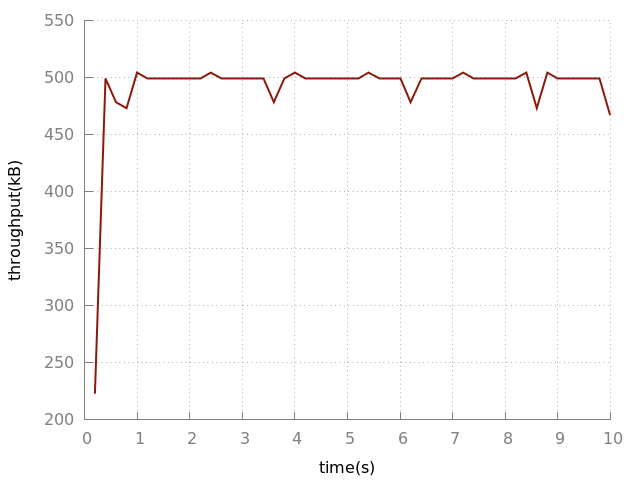
\includegraphics[width=\textwidth]{ftp_throughput.png}
\caption{FTP throughput}
\label{ftp_throughput}
\end{minipage}
\begin{minipage}[b]{0.45\linewidth}
\centering
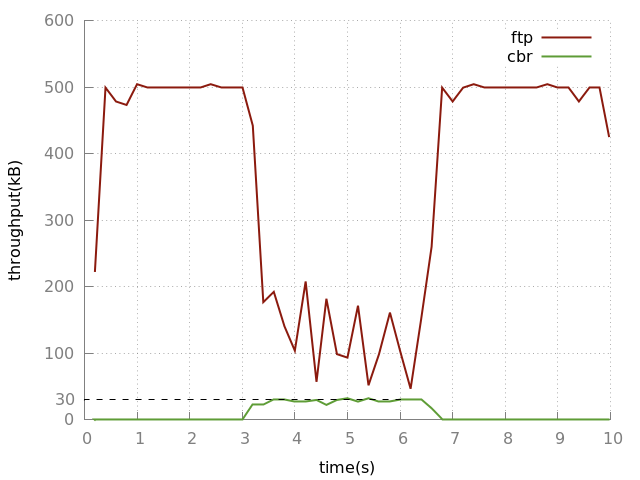
\includegraphics[width=\textwidth]{ftp_cbr_throughput.png}
\caption{FTP \& CBR throughput}
\label{ftp_cbr}
\end{minipage}
\end{figure}

\subsection{Consider now that the model is able to guarantee a certain amount
    of upload bandwidth to every application, which performance do you expect
    for both applications (FTP and CBR)?}
The performance of the FTP application will seem unaffected by the CBR traffic
because it doesn't need alot of upload bandwidth to get the acknowledgements
through.
The CBR application will be slowed down a bit because it can't use all the
available upload bandwidth.

\subsection{What would be the result if bandwidth was even more restricted?
    For example, up to September 2012 KotNet limitations were 512kbps for
    downstream traffic and 100kbps for upstream traffic.}
The FTP application would be slowed down alot.
Not only is the download bandwidth far smaller, but because the download is
slowed down, there have to be more acknowledgements, which requires more
upload bandwidth and that bandwidth is shared with a CBR application.

\subsection{Configure the upload connection with a fixed \emph{rate\_} of 30k.
    Explain the simulated result (no plot required).
    What would be your (extra) solution(s) to improve the download experience
    on shared LANs behind capped Internet connections?
    How could you practically realise this?}
The FTP application is unaffected by the CBR traffic, this is because there's
more than enough upload bandwidth for the CBR traffic and the acknowledgements
combined.
The solution is to try to share bandwidth in a way that is fair.
In this case the network should drop packets from the CBR application, so
there is enough bandwidth available for the acknowledgements.

\subsection{Suppose we have in the future a KotNet/Telenet cable subscription
    that has 10 times more capacity: i.e. a connection that has a downstream
    capacity of 40Mbps with an upstream capacity of 2Mbps.}

\hspace*{\fill}\begin{minipage}{0.94\textwidth}
    \subsubsection{What performance can you expect if there are 10 users behind
        this connection and all performing the same activities as in this
        exercise? Why?}
    The result would be approximately the same as one user on the present
    network, since the amount of users has increased just as much as the
    available capacity.
    In practice the bandwidth would probably not be distributed completely
    fairly, so some users would get slightly more bandwidth, some slightly less.
    
    \subsubsection{What performance can you expect if there are only 5 users
        using the network? Why?}
    Double the current performance.
    There's only five times as many users and ten times as much capacity,
    so every user gets roughly double the previous capacity.
\end{minipage}

\newpage

\section{Tahoe and Reno versus bursty web traffic}

\subsection{Investigate the throughput of the main FTP application.
    Can you indicate the effects the individual bursts of web traffic have
    on its total throughput?
    Why do these effects not immediately become visible when each burst starts
    (i.e. at 5, 10 or resp. 15 seconds)?}
When the first burst of `http' traffic starts, the throughput of the FTP
application drops very fast.
It slowly recovers after each burst but drops fast a few times.
The result is that the FTP throughput is dramatically reduced because of a
few small (2 second) bursts of `http' traffic.
The effect is not immediately visible because the bursts exist of connections
that are started sequentially, the first few connections don't make much of a
difference but when more connections are opened the congestion control kicks in.

\begin{figure}[h]
\centering
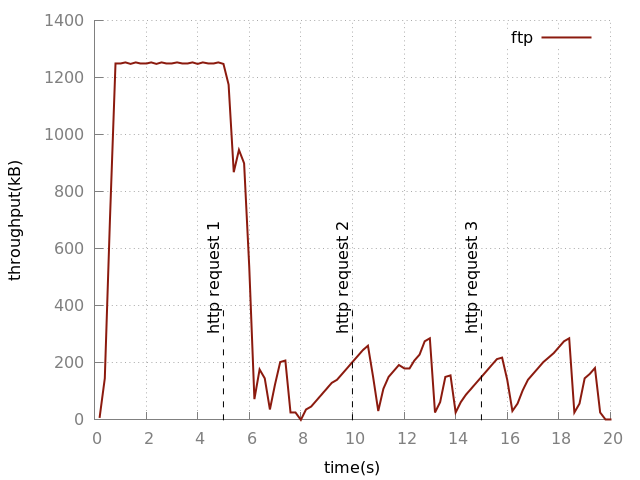
\includegraphics[width=0.6\textwidth]{ftp_3http.png}
\caption{FTP throughput with intermittent http requests}
\label{ftp_3http}
\end{figure}

\subsection{Plot the congestion window size and slow start thresholds in
    another graph.
    Can you identify the different phases of the TCP algorithm?
    When is the slow start threshold recalculated and how?
    Take one `sawtooth' pattern in the graph and indicate a few reasonable
    values for the congestion window on the graph.
    What is the first interval the TCP congestion avoidance algorithm is
    active?}
The slow start threshold is recalculated when a timeout occurs.
The new slow start threshold is set to half of the current slow start threshold.
The first interval wherein the congestion avoidance algorithm is active is
around the $6^{th}$ second.

\begin{figure}[h]
\centering
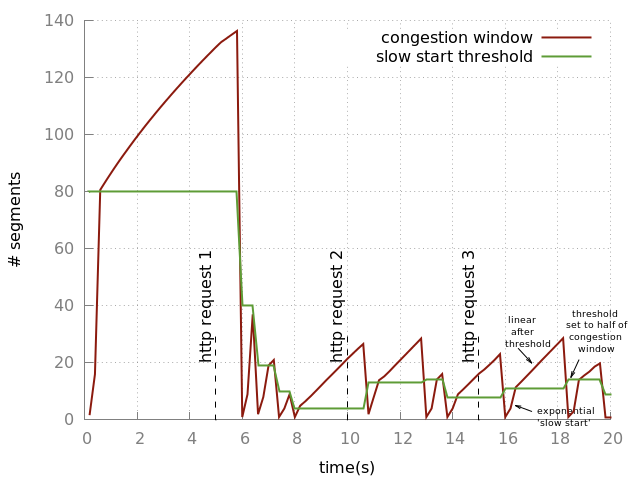
\includegraphics[width=0.6\textwidth]{ftp_3http_wnd_thresh.png}
\caption{Congestion window \& Slow start threshold for TCP Tahoe}
\label{Tahoe}
\end{figure}

\subsection{Change the TCP implementation of the main FTP connection into
    \emph{Reno}.
    Plot the congestion window and slow start thresholds.
    Do you spot the differences with the default TCP \emph{Tahoe}
    implementation?
    Why does the window sometimes still drop to zero?}
Yes the congestion window does not always drop to zero as in TCP Tahoe.
That is an important improvement in TCP Reno, the congestion window starts at
the new slow start threshold instead of falling back to zero.
It still drops to zero sometimes, when the slow start threshold is too small.

\begin{figure}[h]
\centering
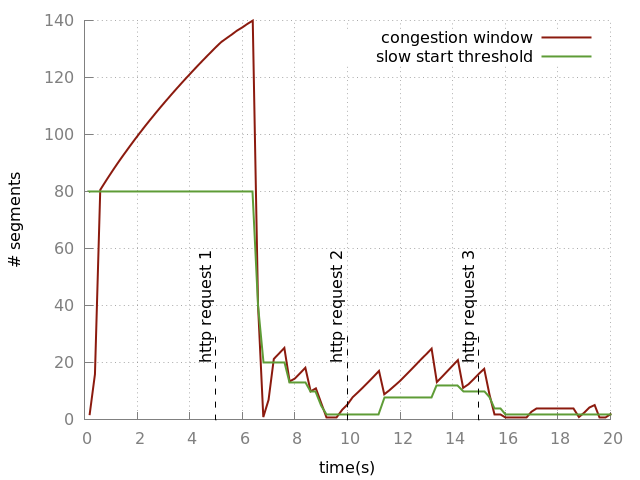
\includegraphics[width=0.6\textwidth]{ftp_3http_wnd_thresh_Reno.png}
\caption{Congestion window \& Slow start threshold for TCP Reno}
\label{Reno}
\end{figure}

\newpage

\lstinputlisting[language=tcl, caption=Source code used for exercise 2]{exercise21.tcl}

\end{document}
